\documentclass[dvipsnames, tikz]{standalone}
\usepackage{amsmath}
\usepackage{arevmath}
\usepackage{xcolor}
\usepackage{tikz}
\usetikzlibrary{calc}
\usetikzlibrary{decorations.pathreplacing,calligraphy,3d}
\usetikzlibrary{matrix,shapes,fit,backgrounds}

\begin{document}
	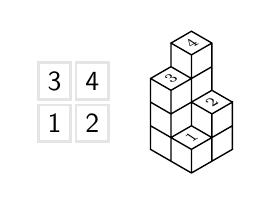
\begin{tikzpicture}[
		%Global config
		>=latex,
		line width=1pt,
		color = black,
		every left delimiter/.style={xshift=1ex},
		every right delimiter/.style={xshift=-1ex},
		%Styles
		Matrix/.style={
			matrix of nodes,
			%text height=2.5ex,
			%text depth=0.75ex,
			%text width=3.25ex,
			%align=center,
			%left delimiter=(,
			%right delimiter=),
			column sep=1pt,
			row sep=1pt,
			nodes={draw=black!10}, % Uncoment to see the square nodes.
			%nodes in empty cells,
		},
		DA/.style={
			fill,
			opacity=0.2,
			rounded corners,
			inner sep=-3pt,
			line width=1pt,
		},
		main/.style={
			line width=0.5pt,
			color=black
			}
		]
		
		\matrix[Matrix] at (0,0) (M){ % Matrix contents  
			\sf 3 & \sf 4\\
			\sf 1 & \sf 2\\ 
		};
	
		\begin{scope}[xshift=1.5cm, yshift=-0.9cm, scale=0.3, font=\tiny]
			\draw[main] (0,0) --++(30:2) --++(0,2) --++(30:-1) --++(0,-2) ++(30:-1) --++(0,1) --++(30:2) ++(0,1) --++(150:1) --++(0,2) --++(150:1) --++(30:-1) --++(-30:1) --++(30:1) ++(30:-1) --++(0,-3) --++(-30:1) ++(0,1) --++(150:1) --++(30:1) ++(0,1) --++(30:-1) --++(150:1) --++(0,1) ++(0,-1)--++(30:-1) --++(0,-3) --++(-30:2) ++(0,1) --++(150:2) ++(0,1) --++(-30:1) --++(30:1) ++(0,1) --++(30:-1) --++(150:1) ++(-30:1) --++(0,-3) ++ (0,1) --++(30:1);
			\path (0,1.5) node[main, rotate=30,xslant=-0.5] {1};
			\path (30:1) ++ (0,2.5) node[main, rotate=30,xslant=-0.5] {2};
			\path (150:1) ++ (0,3.5) node[main, rotate=30,xslant=-0.5] {3};
			\path (0,5.5) node[main, rotate=30,xslant=-0.5] {4};
		\end{scope}
	\end{tikzpicture}
\end{document}